% -----------------------------------------------
% DCC831 - IA Generativa para Música (UFMG, 2026/2)
% Trabalho Final - Geração Musical Simbólica com Redes Neurais Autoregressivas
% Formatado com o template oficial do ISMIR 2026 (github.com/ismir/paper_templates)
% Compilação: tectonic main.tex  (ou pdflatex + bibtex)
% -----------------------------------------------

\documentclass{article}
\usepackage[T1]{fontenc}
\usepackage[utf8]{inputenc}
\usepackage[brazilian]{babel}
\usepackage{ismir} % versão "camera-ready" (sem a opção submission, para exibir os autores)
\usepackage{amsmath,cite,url}
\usepackage{xurl} % permite quebrar a URL do repositório em qualquer ponto
\usepackage{graphicx}
\usepackage{booktabs}
\usepackage{color}

% A nota de copyright do template cita os anais do ISMIR; como este é um trabalho de disciplina, substituímos apenas esse texto
\makeatletter
\renewcommand{\permission}{%
  \begin{figure}[b]{%
    \footnotesize
    {
\includegraphics[alt={CC-BY License},height=0.45cm]{cc_by.pdf}}
    \vskip -.45cm
    \begin{spacing}{1.1}
      \hskip 1.5cm \copyright \hskip .1cm \authorname.
      Licenciado sob Creative Commons Attribution 4.0 International License (CC BY 4.0).
      \textbf{Atribuição:} \authorname,
      ``\removelinebreaks{\@title}'', Trabalho Final de DCC831 -- IA Generativa para Música, UFMG, 2026.
    \end{spacing}
    }
  \end{figure}
}
% rótulos em português (o ismir.sty os define fixos em inglês)
\def\fnum@figure{\textbf{Figura \thefigure}}
\def\fnum@table{\textbf{Tabela \thetable}}
\def\abstract{\begin{center}\bf RESUMO\end{center}}
\def\thebibliography#1{
  \section{Referências}\list
  {[\arabic{enumi}]}{
  \settowidth\labelwidth{[#1]}\leftmargin 1em
  \advance\leftmargin\labelsep
  \usecounter{enumi}
  }
  \def\newblock{\hskip .01em plus .01em minus .01em}
  \sloppy\clubpenalty4000\widowpenalty4000
  \sfcode`\.=1000\relax
}
\makeatother

\newcommand{\repo}{\url{https://github.com/PhPires13/IAGM-TP-Final-Symbolic-Music-Generation-Autoregressive-Neural-Networks}}

\title{Composição Musical Guiada por Curvas de Energia e Tensão com Transformers}

\multauthor
  {Pedro Henrique Gonçalves Pires \hspace{0.5cm} Julia Souza Moura \hspace{0.5cm} Natanael dos Santos}
  {\bfseries{Leonardo Cesar Cota de Castro \hspace{0.5cm} Júlia Borba Fonseca de Souza}\\
   Departamento de Ciência da Computação -- Universidade Federal de Minas Gerais}

\def\authorname{P. H. G. Pires, J. S. Moura, N. dos Santos, L. C. C. de Castro e J. B. F. de Souza}

\sloppy

\begin{document}

\maketitle

\begin{abstract}
Modelos autoregressivos geram música simbólica convincente, mas dão ao usuário pouco controle sobre como a peça evolui no tempo. Propomos um Transformer \emph{decoder-only}, implementado em PyTorch, que compõe piano pop seguindo duas curvas definidas compasso a compasso, uma de \emph{energia} (densidade de notas e intensidade) e outra de \emph{tensão} (notas fora da escala e intervalos dissonantes), além de um quadrante de emoção global. As condições entram como tokens REMI forçados durante a geração, sem mudar a arquitetura. O modelo é pré-treinado no Pop1K7 e ajustado no EMOPIA+, e comparado com uma cadeia de Markov de ordem 4 nos mesmos dados e tokens. No teste, a sobreposição média (OA) de sete métricas do MusPy com as músicas humanas é de 0,927, perto do teto de 0,940 dado pela validação humana, contra 0,622 do Markov. As curvas são seguidas com correlação de Spearman de 0,81 (energia) e 0,48 (tensão); com curvas embaralhadas a correlação cai a zero, o que mostra que o modelo usa o controle. O pré-treino mais que dobra a aderência à tensão (0,20 para 0,48), e o efeito do token de emoção na valência é fraco.
\end{abstract}

\section{Introdução}\label{sec:introducao}

Transformers autoregressivos~\cite{vaswani2017} tornaram-se o modelo dominante para gerar música simbólica, ao tratar a peça como uma sequência de tokens~\cite{huang2019music,huang2020pop}. Gerar ``livremente'', no entanto, é pouco útil para quem compõe: interessa dizer \emph{como} a música deve se desenvolver, por exemplo, começar calma, crescer em intensidade e terminar com tensão harmônica.

A tarefa escolhida é a \textbf{composição condicionada por atributos}: dado um quadrante de emoção e duas curvas, de energia e de tensão, com um nível por compasso, gerar uma peça de piano que as siga. As contribuições são: (i) definições simples e mensuráveis de energia e tensão por compasso, usadas tanto para rotular o treino quanto para avaliar a geração; (ii) um condicionamento só por tokens, que vale igualmente para o Transformer e para o baseline; (iii) uma avaliação que mede, separadamente, a semelhança estatística com a música humana e a \emph{fidelidade ao controle}, incluindo um experimento com curvas embaralhadas que verifica se o modelo de fato usa a condição.

\section{Trabalhos Relacionados}\label{sec:relacionados}

O Music Transformer~\cite{huang2019music} mostrou que a autoatenção captura estrutura musical de longo prazo. O Pop Music Transformer~\cite{huang2020pop} introduziu a representação REMI, com tokens explícitos de compasso e posição, que adotamos; o Compound Word Transformer~\cite{hsiao2021compound} agrupa tokens e publicou o Pop1K7, usado aqui no pré-treino. Sobre emoção, o EMOPIA~\cite{hung2021emopia} rotula clipes de piano pop nos quadrantes do modelo de Russell~\cite{russell1980}, e Huang et al.~\cite{huang2024emotion} geram por emoção em dois estágios e publicaram o EMOPIA+, a versão alinhada ao beat que usamos. O controle por atributos de compasso aparece no MuseMorphose~\cite{wu2023musemorphose} (intensidade rítmica e polifonia) e no FIGARO~\cite{vonrutte2023figaro} (descrições de alto nível por compasso); nossa tensão é uma simplificação dos modelos de tensão tonal de Herremans e Chew~\cite{herremans2016tension}. A avaliação segue Yang e Lerch~\cite{yang2020evaluation}, com métricas do MusPy~\cite{dong2020muspy}, e a tokenização usa o MidiTok~\cite{fradet2021miditok}.

\section{Método}\label{sec:metodo}

\textbf{Dados.} O EMOPIA+ tem 1\,071 clipes de piano pop (4/4, mediana de 18 compassos) com rótulo de quadrante (Q1 alegre, Q2 tenso, Q3 triste, Q4 sereno). Usamos a partição oficial, \textbf{feita por música}, com 869/114/88 clipes em treino/validação/teste; o teste só foi usado na avaliação final. Juntamos as faixas de melodia, textura e baixo numa faixa de piano e descartamos a faixa de anotação de acordes. A versão original do EMOPIA foi abandonada após o primeiro treino: suas notas não estão alinhadas a nenhum pulso (só 9,5\% dos ataques caem perto da grade de semicolcheia, contra 91,3\% no EMOPIA+), e as amostras não tinham ritmo nem tonalidade estáveis. Para o pré-treino usamos o Pop1K7~\cite{hsiao2021compound}, com 1\,747 covers de piano pop (cerca de 108\,h). Como os dois conjuntos vêm do mesmo laboratório, removemos do Pop1K7 toda música que contém mais de 30\% dos 6-gramas de intervalos da linha superior de algum clipe de validação ou teste (o limiar fica acima do percentil 95 entre músicas sabidamente diferentes, 0,09): 3 músicas saíram, sobrando 1\,657 para treino e 87 para validação. O treino do EMOPIA+ é transposto de $-5$ a $+6$ semitons e o Pop1K7 de $-3$ a $+3$.

\textbf{Energia e tensão.} Uma única função mede cada compasso, usada para rotular o treino e avaliar as músicas geradas. A \emph{energia} é a média da densidade de notas (ataques por compasso divididos por 40, limitado a 1) e da velocity média normalizada. A \emph{tensão} é a média da fração de notas fora da escala da tonalidade da peça (estimada por Krumhansl--Schmuckler~\cite{krumhansl1990}) e da fração de pares de notas simultâneas em intervalo dissonante (2\textsuperscript{a}, trítono ou 7\textsuperscript{a}). Cada atributo é quantizado em $K=3$ níveis pelos tercis do treino do EMOPIA+ (limites 0,360 e 0,497 para energia; 0,067 e 0,145 para tensão), o que deixa os níveis balanceados (33/33/33\%) e pouco correlacionados entre si (Spearman 0,15).

\textbf{Representação.} Usamos REMI~\cite{huang2020pop} via MidiTok, com 12 posições por tempo (a grade de 1/12 de tempo captura as tercinas, presentes em 7\% dos ataques que a grade de 1/4 perde). REMI foi escolhido porque o token \texttt{Bar} marca o início de cada compasso, exatamente onde a condição entra. Cada peça vira
\texttt{BOS Emotion\_Q$x$ Bar Energy\_$e$ Tension\_$t$} \emph{notas} \texttt{Bar}~\ldots~\texttt{EOS}, com \texttt{Emotion\_None} no Pop1K7, que não tem rótulo. O vocabulário tem \textbf{326 tokens}, e as sequências têm em média \textbf{975 tokens} por clipe no treino do EMOPIA+ (1\,021 na validação, 943 no teste) e 4\,957 por música no Pop1K7. As janelas de treino têm o tamanho do contexto do modelo, com passo de metade dele, e toda janela recebe \texttt{BOS Emotion} na frente, para que a emoção nunca saia do contexto.

\textbf{Modelo.} O Transformer \emph{decoder-only} usa embedding de tokens e posicional aprendido, camadas \texttt{nn.TransformerEncoderLayer} com pré-normalização e máscara causal, normalização final e cabeça linear com pesos amarrados ao embedding. O modelo grande tem 6 camadas, $d_{\text{model}}=512$, 8 cabeças e contexto de 1\,024 (19,6\,M parâmetros); o pequeno tem 4 camadas, $d_{\text{model}}=256$, 4 cabeças e contexto de 512 (3,4\,M). O treino minimiza a entropia cruzada do próximo token com AdamW ($\beta=(0{,}9;\,0{,}95)$, decaimento 0,1), lote de 32 (grande) ou 64 (pequeno), \emph{warmup} linear, decaimento cosseno até 10\% da taxa inicial, \emph{gradient clipping} em 1,0 e parada antecipada pela perda de validação. O pré-treino usa taxa de $3\cdot10^{-4}$ (grande) ou $5\cdot10^{-4}$ (pequeno), com 2\,000 passos de \emph{warmup} e paciência 3; o ajuste fino no EMOPIA+ parte desses pesos com taxa de $10^{-4}$, 100 passos de \emph{warmup} e paciência 3. Como ablação, os dois tamanhos também são treinados do zero no EMOPIA+, com as taxas do pré-treino e paciência 5.

\textbf{Baseline.} Uma cadeia de Markov de ordem $n$ sobre \emph{os mesmos tokens}, com desconto absoluto interpolado~\cite{ney1994}, ajustada nos mesmos dados que o Transformer viu (Pop1K7 e treino do EMOPIA+, 18,2\,M tokens). A ordem e o desconto foram escolhidos pela verossimilhança na validação: $n=4$, $D=0{,}9$.

\textbf{Geração e amostragem.} O modelo e o baseline expõem a mesma interface (logits do próximo token dado o prefixo), então a rotina de geração é a mesma: os tokens \texttt{BOS} e \texttt{Emotion} abrem a sequência e, a cada \texttt{Bar} gerado, os tokens \texttt{Energy} e \texttt{Tension} do compasso são \emph{forçados}, até a curva acabar. A amostragem própria aplica temperatura, top-$k$ e top-$p$~\cite{holtzman2020}.

\section{Experimentos}\label{sec:experimentos}

Os modelos foram treinados numa GPU NVIDIA L40S com bf16: o pré-treino grande leva cerca de 32\,min e uma época de ajuste fino, 41\,s. A amostragem foi escolhida na \emph{validação}, numa grade de temperatura $\in\{0{,}8;\,0{,}9;\,1{,}0\}$ e top-$p\in\{0{,}9;\,0{,}95;\,1{,}0\}$, pela maior OA média entre as configurações que seguem as duas curvas: $T=0{,}9$ e top-$p=1{,}0$, aplicada a todos os sistemas.

No teste, cada sistema gera \textbf{100 peças}, cada uma com a curva e o quadrante reais de um clipe de teste (a mesma lista para todos os sistemas). Avaliamos três aspectos:
(i) \textbf{semelhança com a música humana}: sete métricas do MusPy (extensão de alturas, n.\textsuperscript{o} de classes de altura, entropia de classes de altura, consistência de escala, polifonia, taxa de tempos vazios e consistência rítmica), comparando a \emph{distribuição} de cada sistema com a dos 88 clipes humanos de teste pela área de sobreposição (OA) e pela divergência KL entre estimativas de densidade por kernel~\cite{yang2020evaluation}; a validação humana contra o teste humano dá o teto esperado;
(ii) \textbf{fidelidade ao controle}: os níveis de energia e tensão de cada compasso gerado são medidos pela mesma função do treino e comparados aos pedidos (acurácia exata, acurácia com tolerância de $\pm1$ nível e correlação de Spearman $\rho$); a mesma medição contra curvas \emph{embaralhadas} entre peças (permutação com seed fixa) dá o nível do acaso;
(iii) \textbf{emoção}: sem um classificador, usamos a energia média como indicador de excitação (Q1, Q2 $>$ Q3, Q4) e a fração de peças em modo maior como indicador de valência (Q1, Q4 $>$ Q2, Q3).

\section{Resultados e Discussão}\label{sec:resultados}

\begin{table}[t]
  \centering
  \footnotesize
  \setlength{\tabcolsep}{3.5pt}
  \begin{tabular}{@{}lccc@{}}
    \toprule
    Execução & Parâm. & Perda val. & Perplexidade \\
    \midrule
    Pré-treino grande (Pop1K7) & 19,6\,M & 1,537 & 4,65 \\
    Pré-treino pequeno (Pop1K7) & 3,4\,M & 1,574 & 4,83 \\
    \midrule
    \textbf{Ajuste fino grande} & 19,6\,M & \textbf{1,561} & \textbf{4,76} \\
    Ajuste fino pequeno & 3,4\,M & 1,614 & 5,02 \\
    Do zero, grande & 19,6\,M & 2,127 & 8,39 \\
    Do zero, pequeno & 3,4\,M & 1,906 & 6,72 \\
    Markov ($n=4$) & -- & 3,248 & 25,7 \\
    \bottomrule
  \end{tabular}
  \caption{Perda e perplexidade na melhor época, na validação do Pop1K7 (pré-treino) ou do EMOPIA+ (demais).}
  \label{tab:treino}
\end{table}

\begin{figure}[t]
  \centering
  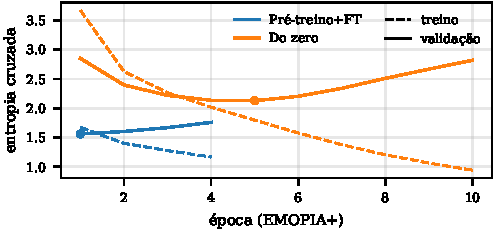
\includegraphics[width=\columnwidth]{figuras/treino.pdf}
  \caption{Curvas de treino e validação no EMOPIA+ dos modelos grandes. O ponto marca a melhor época.}
  \label{fig:treino}
\end{figure}

\textbf{Treino.} O pré-treino é o fator decisivo (Tabela~\ref{tab:treino}, Figura~\ref{fig:treino}). Do zero, o modelo grande decora o EMOPIA+ (perda de treino 0,94 contra 2,82 na validação na época 10) e fica pior que o pequeno. Com pré-treino, a ordem se inverte: a perplexidade do grande cai de 8,39 para 4,76, e a melhor época de ajuste fino já é a primeira, ou seja, quase todo o ganho vem do Pop1K7. O Markov fica muito atrás (25,7).

\begin{table}[t]
  \centering
  \footnotesize
  \setlength{\tabcolsep}{3pt}
  \begin{tabular}{@{}lccccc@{}}
    \toprule
    Sistema & Classes & OA entr. & OA esc. & OA rit. & OA média \\
    \midrule
    Humano (teste) & 8,43 & -- & -- & -- & -- \\
    Humano (val., teto) & 8,45 & 0,978 & 0,896 & 0,953 & 0,940 \\
    \midrule
    \textbf{Pré-treino + AF, gr.} & 8,65 & 0,826 & 0,928 & 0,961 & \textbf{0,927} \\
    Pré-treino + AF, peq. & 8,87 & 0,820 & 0,939 & 0,968 & \textbf{0,929} \\
    Do zero, grande & 10,18 & 0,816 & 0,861 & 0,937 & 0,896 \\
    Do zero, pequeno & 10,18 & 0,859 & 0,834 & 0,939 & 0,898 \\
    Markov & 12,00 & 0,165 & 0,116 & 0,870 & 0,622 \\
    \bottomrule
  \end{tabular}
  \caption{Semelhança com o teste humano (100 peças por sistema). ``Classes'': média do n.\textsuperscript{o} de classes de altura usadas. OA (maior é melhor) da entropia de classes de altura, da consistência de escala e da consistência rítmica; a média é sobre as sete métricas. As tabelas completas, com média, desvio e KL, estão no repositório.}
  \label{tab:oa}
\end{table}

\begin{figure}[t]
  \centering
  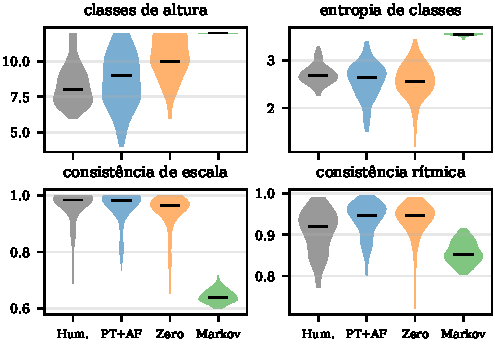
\includegraphics[width=\columnwidth]{figuras/violinos.pdf}
  \caption{Distribuição de quatro métricas no teste (100 peças por sistema). PT+AF: pré-treino + ajuste fino; Zero: treinado do zero (ambos grandes). Hum.: humano. O traço marca a mediana.}
  \label{fig:violinos}
\end{figure}

\textbf{Semelhança com a música humana.} Os modelos com pré-treino ficam a cerca de 0,01 do teto humano na OA média (Tabela~\ref{tab:oa}). O pré-treino corrige justamente a tonalidade: do zero, o modelo usa em média 10,2 classes de altura por clipe, um cromatismo errante, contra 8,4 nos humanos e 8,7 com pré-treino, e a OA da consistência de escala sobe de 0,86 para 0,93 (Figura~\ref{fig:violinos}). O Markov não tem centro tonal: usa as 12 classes em todas as peças, com entropia de 3,54 bits, perto do máximo $\log_2 12 = 3{,}58$, porque um 4-grama de tokens REMI enxerga pouco mais de uma nota (\texttt{Pitch Velocity Duration}). O ritmo do Markov, por outro lado, é razoável (OA de 0,95 na polifonia e 0,90 em tempos vazios).

\begin{table}[t]
  \centering
  \footnotesize
  \setlength{\tabcolsep}{3pt}
  \begin{tabular}{@{}llcccccc@{}}
    \toprule
    & & \multicolumn{3}{c}{Energia} & \multicolumn{3}{c}{Tensão} \\
    \cmidrule(lr){3-5}\cmidrule(l){6-8}
    Sistema & Curva & exata & $\pm1$ & $\rho$ & exata & $\pm1$ & $\rho$ \\
    \midrule
    \textbf{PT + AF, gr.} & pedida & 0,75 & 1,00 & 0,81 & \textbf{0,54} & \textbf{0,91} & \textbf{0,48} \\
                         & embar. & 0,33 & 0,77 & 0,00 & 0,37 & 0,76 & 0,01 \\
    PT + AF, peq.        & pedida & \textbf{0,79} & 1,00 & \textbf{0,84} & 0,53 & 0,88 & 0,42 \\
    Do zero, gr.         & pedida & 0,71 & 0,99 & 0,78 & 0,45 & 0,82 & 0,20 \\
    Do zero, peq.        & pedida & 0,70 & 0,99 & 0,76 & 0,41 & 0,82 & 0,20 \\
    Markov               & pedida & 0,33 & 0,77 & $-$0,04 & 0,33 & 0,67 & 0,03 \\
    \bottomrule
  \end{tabular}
  \caption{Fidelidade às curvas, compasso a compasso, no teste. ``Embar.'': a mesma geração comparada com curvas de outras peças (nível do acaso). Com $K=3$ níveis, o acaso dá cerca de 0,33 de acurácia exata.}
  \label{tab:fidelidade}
\end{table}

\begin{figure}[t]
  \centering
  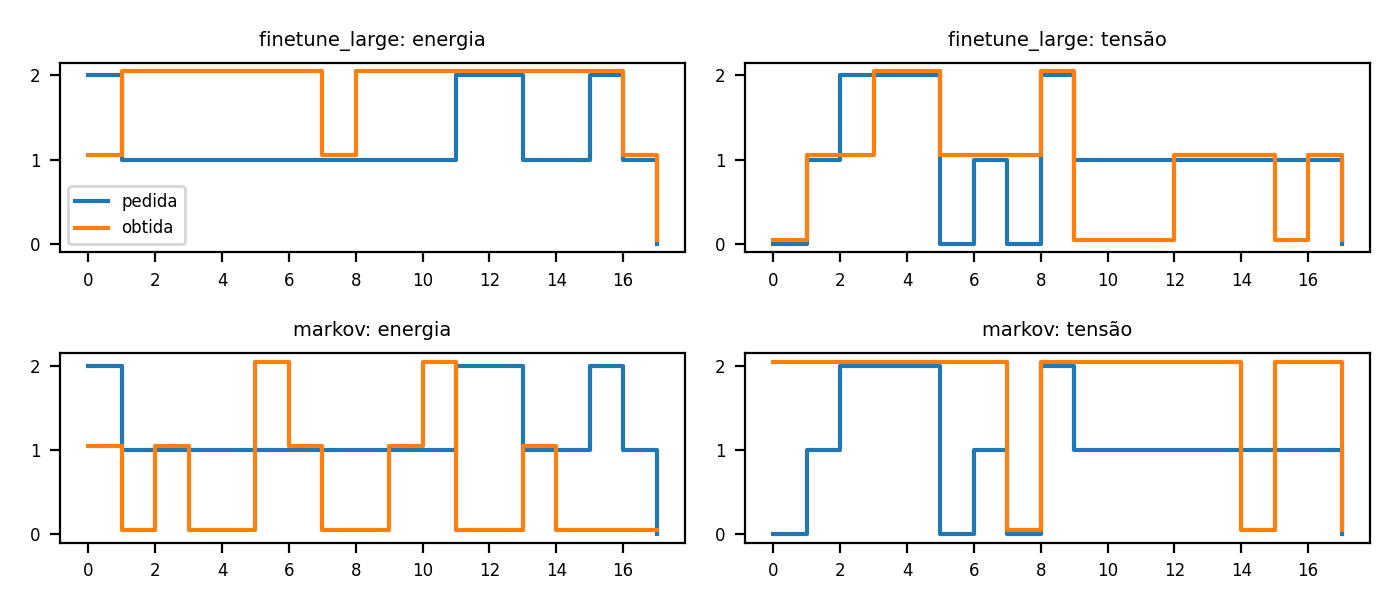
\includegraphics[width=\columnwidth]{figuras/curvas_controle.png}
  \caption{Curva pedida (azul) e obtida (laranja) na peça de teste \texttt{000} (quadrante Q1), para o Transformer com pré-treino (acima) e o Markov (abaixo). Eixo $x$: compasso; eixo $y$: nível.}
  \label{fig:curvas}
\end{figure}

\textbf{Fidelidade ao controle.} Os controles funcionam (Tabela~\ref{tab:fidelidade}, Figura~\ref{fig:curvas}). Com a curva pedida, a correlação é de 0,81 na energia e 0,48 na tensão; contra uma curva embaralhada, cai para zero, então o modelo segue a curva pedida, e não uma curva média. A energia é fácil, e já sai bem do zero ($\rho=0{,}78$); a tensão é difícil e é onde o pré-treino mais ajuda, mais que dobrando a correlação (0,20 para 0,48), o que é coerente com a tensão depender de harmonia, que é o que o Pop1K7 ensina. O Markov ignora as curvas: com contexto de 3 tokens, o token de controle sai do alcance logo depois do início do compasso. Na escolha da amostragem, temperaturas mais baixas ou top-$p<1$ pioram as duas coisas: a música empobrece (extensão de 32 contra 50 semitons dos humanos com $T=0{,}8$, top-$p=0{,}9$) e a aderência à tensão cai ($\rho=0{,}26$), indicando que o modelo está bem calibrado e não precisa de truncamento.

\textbf{Emoção.} A energia média reproduz a separação humana de excitação entre Q1/Q2 e Q3/Q4 (diferença de $+0{,}18$ no modelo e nos humanos; $-0{,}01$ no Markov). Esse efeito, porém, pode vir da curva de energia, que foi tirada de um clipe do mesmo quadrante, e não do token de emoção. O teste real do token é a valência, e o efeito é fraco: a diferença na fração de peças em modo maior entre Q1/Q4 e Q2/Q3 é de $+0{,}11$, contra $+0{,}51$ nos humanos; por exemplo, 37\% das peças Q2 (tensas) saem em modo maior, contra 16\% nos humanos. Com cerca de 870 clipes rotulados e um pré-treino todo sem rótulo, o modelo aprende pouco a associar quadrante a modo.

\textbf{Análise qualitativa.} O repositório traz, em \texttt{samples/}, cinco pedidos sorteados com seed fixa, cada um gerado pelo Transformer e pelo Markov, junto com o clipe humano de onde veio a curva, em MIDI e em áudio sintetizado (piano, 120\,BPM). Dois integrantes ouviram os 15 áudios e deram notas de 1 a 3 a cada sistema, com o humano como referência, em tonalidade, melodia e frase, aderência à curva e emoção: o Transformer teve médias de 1,9, 1,8, 2,5 e 2,6, e o Markov, de 1,0, 1,0, 1,7 e 1,4. Os dois apontaram a mesma melhor peça, a \texttt{035} (nota máxima em tudo: melodia suave, sem notas repetidas), e a mesma pior, a \texttt{031}, que se repete no início antes de progredir; na \texttt{014} também notaram notas repetidas em sequência e, na \texttt{081}, uma nota desafinada perto do fim. A escuta confirma a tonalidade medida: a consistência de escala do Transformer fica entre 0,82 e 1,00 (humanos: 0,96 a 0,99), e o Markov, que usa as 12 classes de altura (0,64 a 0,69), soa sem centro tonal. Já o ritmo do Markov, razoável pelas métricas, foi descrito como sem pulso e cheio de pausas. A estrutura de frase varia: algumas peças do Transformer formam ideias coerentes, outras soam desconexas. Na emoção, os ouvintes julgaram o caráter compatível com o quadrante na maioria das peças, inclusive na \texttt{081} (Q4), estimada em menor; com dois ouvintes e cinco peças, isso não contradiz o efeito fraco na valência, mas indica que o modo é um indicador grosseiro da emoção.

\section{Conclusão}\label{sec:conclusao}

Mostramos que um Transformer pequeno, condicionado apenas por tokens forçados, compõe piano pop que segue curvas de energia e tensão definidas pelo usuário, mantendo estatísticas próximas às da música humana, enquanto uma cadeia de Markov nos mesmos dados não segue as curvas nem mantém a tonalidade. Os dois achados principais são que a qualidade dos dados importa mais que o modelo (o EMOPIA original, sem alinhamento ao beat, inviabilizava o ritmo) e que o pré-treino num conjunto maior é o que dá ao modelo a harmonia necessária para controlar a tensão.

Entre as limitações estão: atributos simplificados (uma tonalidade por peça, sem modulação); o efeito fraco do token de emoção na valência e a confusão entre emoção e curva na excitação; uma avaliação perceptual apenas preliminar, com dois ouvintes do próprio grupo; e a ausência de tokens de andamento. Como trabalhos futuros, propomos isolar o efeito do token de emoção gerando com a mesma curva e quadrantes diferentes, usar medidas de tensão tonal mais ricas~\cite{herremans2016tension}, fazer um teste de audição com ouvintes externos e criar uma interface em que o usuário desenhe as curvas. O código, os dados de avaliação e as amostras estão em \repo.

\bibliography{referencias}

\end{document}
